% Information about the beamer-poster template:

%%%%%%%%%%%%%%%%%%%%%%%%%%%%%%%%%%%%%%%%%
% Jacobs Landscape Poster
% LaTeX Template
% Version 1.1 (14/06/14)
%
% Created by:
% Computational Physics and Biophysics Group, Jacobs University
% https://teamwork.jacobs-university.de:8443/confluence/display/CoPandBiG/LaTeX+Poster
%
% Further modified by:
% Nathaniel Johnston (nathaniel@njohnston.ca)
%
% This template has been downloaded from:
% http://www.LaTeXTemplates.com
%
% License:
% CC BY-NC-SA 3.0 (http://creativecommons.org/licenses/by-nc-sa/3.0/)
%
%%%%%%%%%%%%%%%%%%%%%%%%%%%%%%%%%%%%%%%%%
 
%----------------------------------------------------------------------------------------
%       PACKAGES AND OTHER DOCUMENT CONFIGURATIONS
%----------------------------------------------------------------------------------------
 
\documentclass[final]{beamer}
 
\usepackage[scale=1.24]{beamerposter} % Use the beamerposter package for laying out the poster
 
\usetheme{confposter} % Use the confposter theme supplied with this template
 
\setbeamercolor{block title}{fg=ngreen,bg=white} % Colors of the block titles
\setbeamercolor{block body}{fg=black,bg=white} % Colors of the body of blocks
\setbeamercolor{block alerted title}{fg=white,bg=dblue!70} % Colors of the highlighted block titles
\setbeamercolor{block alerted body}{fg=black,bg=dblue!10} % Colors of the body of highlighted blocks
% Many more colors are available for use in beamerthemeconfposter.sty
 
%-----------------------------------------------------------
% Define the column widths and overall poster size
% To set effective sepwid, onecolwid and twocolwid values, first choose how many columns you want and how much separation you want between columns
% In this template, the separation width chosen is 0.024 of the paper width and a 4-column layout
% onecolwid should therefore be (1-(# of columns+1)*sepwid)/# of columns e.g. (1-(4+1)*0.024)/4 = 0.22
% Set twocolwid to be (2*onecolwid)+sepwid = 0.464
% Set threecolwid to be (3*onecolwid)+2*sepwid = 0.708
 
\newlength{\sepwid}
\newlength{\onecolwid}
\newlength{\twocolwid}
\newlength{\threecolwid}
\setlength{\paperwidth}{48in} % A0 width: 46.8in
\setlength{\paperheight}{36in} % A0 height: 33.1in
\setlength{\sepwid}{0.024\paperwidth} % Separation width (white space) between columns
\setlength{\onecolwid}{0.22\paperwidth} % Width of one column
\setlength{\twocolwid}{0.464\paperwidth} % Width of two columns
\setlength{\threecolwid}{0.708\paperwidth} % Width of three columns
\setlength{\topmargin}{-0.5in} % Reduce the top margin size
%-----------------------------------------------------------
 
\usepackage{iipr_beamer}
\usefonttheme{serif}
\usepackage{booktabs} % Top and bottom rules for tables
 
%________________HYPERREFERENCES________________

%\usepackage[colorlinks]{hyperref}        % Hyperreferences (sometimes causes problems, load last)
\definecolor{myblue}{rgb}{0,0.2,0.6}    % Link colour: My own blue
\definecolor{mygreen}{rgb}{0,0.6,0.1} % Link colour: My own green
\definecolor{myred}{rgb}{0.9,0,0.2}     % Link colour: My own red
\hypersetup{colorlinks,breaklinks,urlcolor=myblue,citecolor=myred} % Set link colors throughout the document
%Two ways to make references: \hyperrref[teoremaFundamental]{teorema visto antes} o \ref{teoremaFundamental}
%For hyperlinks: \href{https://www.google.es/}{here}
%For the bibliography: \cite{FerGam}

%----------------------------------------------------------------------------------------
%       TITLE SECTION
%----------------------------------------------------------------------------------------

\title{Complexity Analysis of Polynomial Algorithms\\
\vspace{1cm}
\large{Final Degree Project - Double Degree in Mathematics and Computer Science,\\ \vspace{0.5cm}
Complutense University of Madrid (UCM).
}
} % Poster title
 
\author{Ignacio Iker Prado Rujas} % Author(s)
 
\institute{ \textbf{Tutors:}
	Juan R. Delgado, Jos\'e F. Fernando \textit{\&} Jos\'e M. Gamboa - 
	Department of Algebra, Faculty of Mathematics.} % Institution(s)

%----------------------------------------------------------------------------------------


\begin{document}
 
\addtobeamertemplate{block end}{}{\vspace*{2ex}} % White space under blocks
\addtobeamertemplate{block alerted end}{}{\vspace*{2ex}} % White space under highlighted (alert) blocks
 
\setlength{\belowcaptionskip}{2ex} % White space under figures
\setlength\belowdisplayshortskip{2ex} % White space under equations
 
\begin{frame}[t] % The whole poster is enclosed in one beamer frame
 
\tikz [remember picture,overlay]
    \node at (10,10.5)
        {
\includegraphics[scale=3.75]{ucm.eps}};

\vspace{-2.0cm}
\begin{columns}[t] % The whole poster consists of three major columns, the second of which is split into two columns twice - the [t] option aligns each column's content to the top
 
\begin{column}{\sepwid}\end{column} % Empty spacer column
 
\begin{column}{\onecolwid} % The first column
 
%----------------------------------------------------------------------------------------
%       OBJECTIVES
%----------------------------------------------------------------------------------------
 
\begin{alertblock}{Abstract}

In this work we gather three different proofs appearing in \cite{fg}, \cite{fgu} and \cite{fu1} of the following result: let $R$ be a real closed field and consider the open quadrant $\Qu:=\{x>0,y>0\}\subset R^2$. Then, there exists a polynomial map $f:R^2\to R^2$ such that $f(R^2)=\Qu$. In addition, we compare the computational complexity of the three maps $f$ satisfying the equality $f(R^2)=\Qu$ looking for the most efficient one, and we present 3 new candidates to solve this problem.

\end{alertblock}
 \vspace{-0.3cm}

%----------------------------------------------------------------------------------------
%       INTRODUCTION
%---------------------------------------------------------------------------------------- 

\begin{block}{Introduction}
 
Let $R$ be a real closed field. A very famous theorem by Tarski and Seidenberg (1951) states the following:\vspace{0.4cm}

\textbf{Theorem 1}.
The image of every polynomial map $f:R^m\to R^n$ is a \hyperref[semialgSet]{semialgebraic subset} of $R^n$.
\vspace{0.4cm}
 
In this work we study a sort of converse of this statement proposed by J.M. Gamboa in the 1990 \emph{Oberwolfach Reelle algebraische Geometrie} week:
\vspace{0.4cm}

\textbf{`Inverse problem'}. 
Characterize the semialgebraic subsets of $R^n$ that are polynomial images of some $R^m$.
\vspace{0.4cm}

This problem has its origin in examples such as that $(0,+\infty)$ \textbf{is not} the image of any polynomial map $\R\to\R$, although 
there exists a certain polynomial map $\R^2\to\R^2$ having $\H:=\set{y>0}\subset\R^2$ as its image.
\vspace{-1.3cm}
\end{block}

%----------------------------------------------------------------------------------------
%       MAIN RESULTS
%---------------------------------------------------------------------------------------- 
\begin{block}{Main results}
The main results that we prove are:
\vspace{0.4cm}

\textbf{Theorem 2.}
Let $n\ge2$. For every finite set $F\subset R^n$, the semialgebraic set $R^n\setminus F$ is a polynomial image of $R^n$.
\vspace{0.4cm}

\textbf{Theorem 3.}
Let $n\ge 2$. Given independent linear forms $h_1,\dots,h_r$ of $R^n$, the open semialgebraic set $\set{h_1>0,\dots,h_r>0}$ is a polynomial image of $R^n$.
\vspace{0.4cm}

\textbf{Theorem 4} (Open quadrant $\Qu$ problem).
The open quadrant $\Qu:=\{x>0,y>0\}$ is a polynomial image of $R^2$.


\end{block}
 
%------------------------------------------------
 
 
%----------------------------------------------------------------------------------------
 
\end{column} % End of the first column
 
\begin{column}{\sepwid}\end{column} % Empty spacer column
 
\begin{column}{\twocolwid} % Begin a column which is two columns wide (column 2)
 
\begin{columns}[t,totalwidth=\twocolwid] % Split up the two columns wide column
 
\begin{column}{\onecolwid}\vspace{-.6in} % The first column within column 2 (column 2.1)
 
\vspace{-1cm}
%----------------------------------------------------------------------------------------
%       FIRST PROOF
%----------------------------------------------------------------------------------------
 
\begin{block}{About the first proof}

On the topic of finding a polynomial map $f:\R^2\to\R^2$ verifying Theorem 4, a ``major difficulty''  is that 
\textbf{the closure of its image must contain the positive half-axes}. 
Aiming at this, we approach the positive half-axes with certain families of curves: 
$\alpha_{\lambda}, \beta_{\mu}: \R \to \R^2$. The map $g := (\F, \G)$ defined as:
\begin{equation*}\label{eq:firstMap}
\boxed{
\begin{aligned}
\F({\tt x},{\tt y})&=(1-{\tt x}^3{\tt y}+{\tt y}-{\tt x}{\tt y}^2)^2+({\tt x}^2{\tt y})^2, \\
\G({\tt x},{\tt y})&=(1-{\tt x}{\tt y}+{\tt x}-{\tt x}^4{\tt y})^2+({\tt x}^2{\tt y})^2, \\
\end{aligned}
}
\end{equation*}
behaves well along those curves, namely:
$$
\lim_{s\rightarrow 0} \P(\alpha_{\lambda}(s))=(\lambda^2,0)\ \ \text{and}\ \ \lim_{s\rightarrow 0} \P(\beta_{\mu}(s))=(0,\mu^2).
$$


\end{block}
 
%----------------------------------------------------------------------------------------
 
\end{column} % End of column 2.1

\begin{column}{\onecolwid}\vspace{-.6in} % The second column within column 2 (column 2.2)

\vspace{-1cm}
%----------------------------------------------------------------------------------------
%       THIRD PROOF
%----------------------------------------------------------------------------------------
 
\begin{block}{About the third proof}
 
 The map ${\scalebox{1.5}{$\FFF$}}:= ({\scalebox{1.5}{$\FFF$}}_1, {\scalebox{1.5}{$\FFF$}}_2):\R^2\to\R^2$ defined as:
\begin{equation*}\label{eq:thirdMap}
\boxed{
\begin{aligned}
{\scalebox{1.5}{$\FFF$}}_1({\tt x}, {\tt y}) = ({\tt x}^2{\tt y}^4+{\tt x}^4{\tt y}^2-{\tt y}^2-1)^2+{\tt x}^6{\tt y}^4,\\
{\scalebox{1.5}{$\FFF$}}_2(\x, \y) = ({\tt x}^6{\tt y}^2+{\tt x}^2{\tt y}^2-{\tt x}^2-1)^2+{\tt x}^6{\tt y}^4,
\end{aligned}
}
\end{equation*}
can be expressed as ${\scalebox{1.5}{$\FFF$}} = f_2 \circ f_1$, with
$f_1(\x,\y)=\big(\x^2,\,\y^2\big)$.
This map verifies $f_1\big(\R^2\big)=\overline{\Qu}$,
so given $a,b>0$, we must provide $x,y\ge0$ such that:
\begin{equation*}
\left\{
\begin{aligned}
f_{2,1}(x,y)=a,\\
f_{2,2}(x,y)=b.\\
\end{aligned}
\right.
\end{equation*}
The proof is reduced to check that the boundaries of two certain topological subspaces of $\R^3$ homeomorphic to a closed disc meet $g(\overline{\Qu})$, where $f_2=h\circ g$.

\end{block}
 
%----------------------------------------------------------------------------------------
 
\end{column} % End of column 2.2
 
\end{columns} % End of the split of column 2 - any content after this will now take up 2 columns width

 \vspace{-1cm}

%----------------------------------------------------------------------------------------
%       PICS
%----------------------------------------------------------------------------------------

\begin{alertblock}{Some important graphs regarding the computational analysis}
\begin{center}

\begin{figure}
\vspace{-0.2cm}
\begin{subfigure}{.28\linewidth}\centering
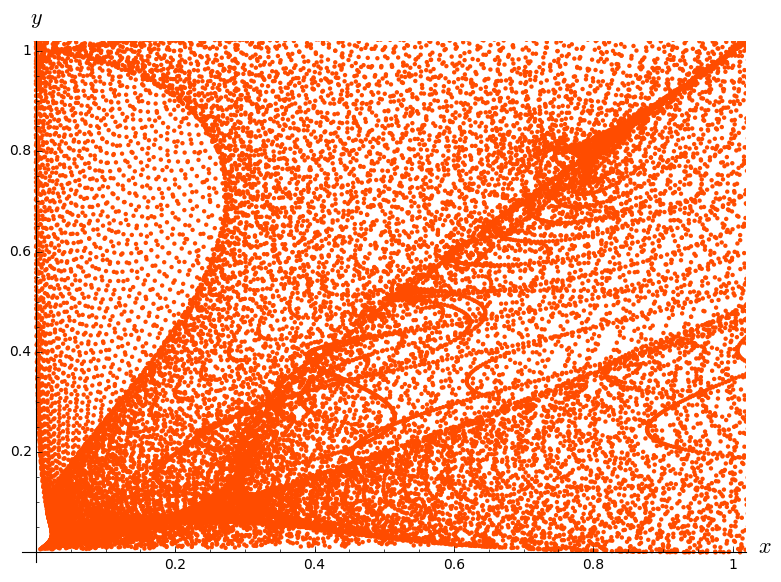
\includegraphics[width=1\textwidth]{plots/ch5_17_P6prime.png}
\vspace{-0.1cm}\caption{$g(\PP_6) \leadsto 1633.50$ s.}
\end{subfigure}
\hspace{2cm}
\begin{subfigure}{.28\linewidth}\centering
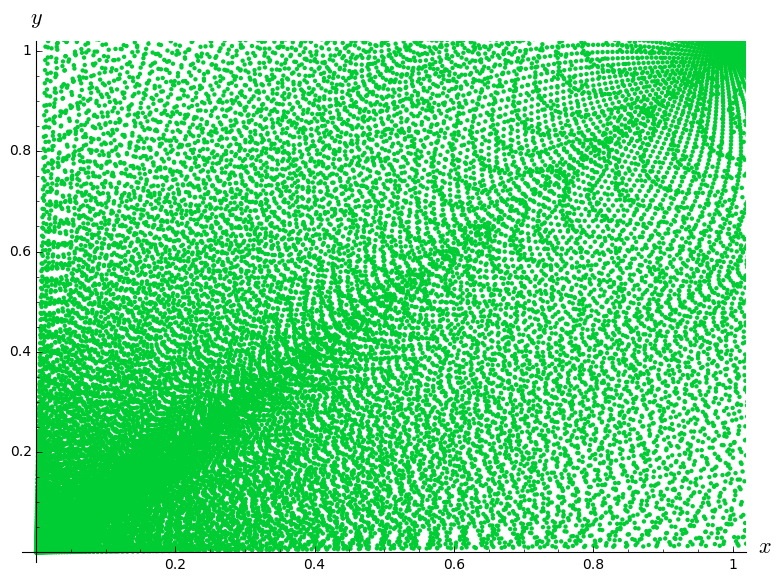
\includegraphics[width=1\textwidth]{plots/ch5_new1_P6prime.png}
\vspace{-0.1cm}\caption{$\mathcal{N}_1(\PP_6) \leadsto 610.06$ s.}
\end{subfigure}
\hspace{2cm}
\begin{subfigure}{.28\linewidth}\centering
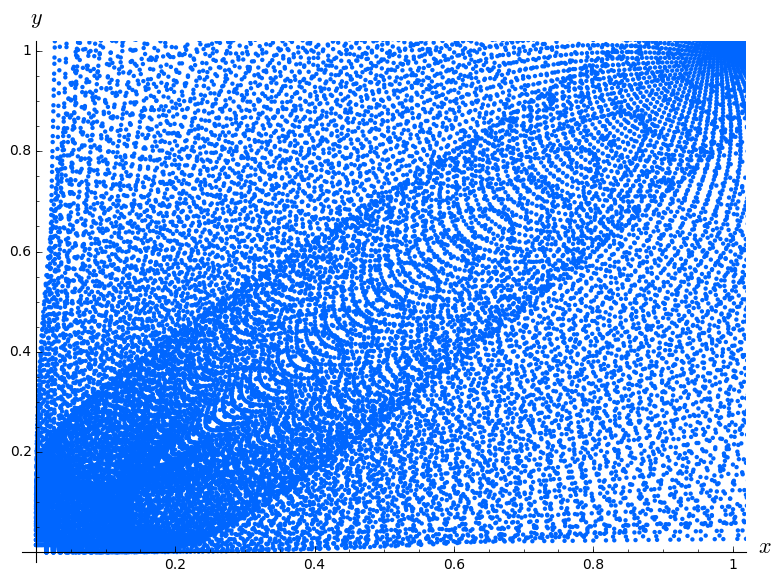
\includegraphics[width=1\textwidth]{plots/ch5_new3_P6.png}
\vspace{-0.1cm}\caption{$\mathcal{N}_3(\PP_6)\leadsto 615.09$ s.}
\end{subfigure}\\[1ex]

%\vspace{-0.1cm}
\begin{subfigure}{.28\linewidth}\centering
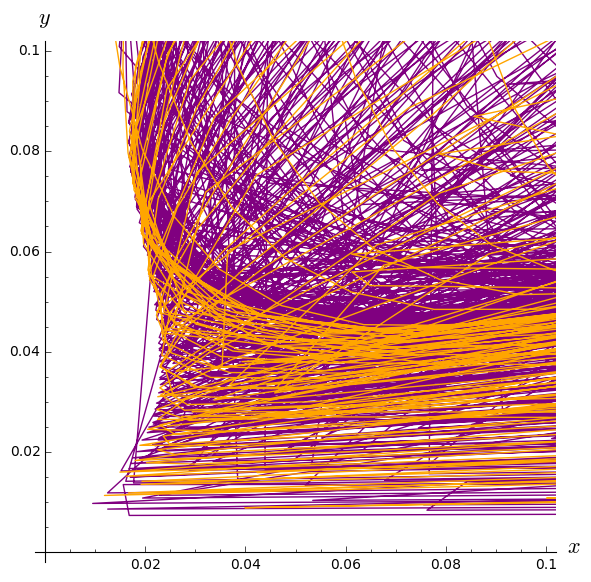
\includegraphics[width=1\textwidth]{plots/ch5_26_1curves4.png}
\vspace{-0.1cm}\caption{$g(\alpha_{\lambda})$ and $g(\beta_{\mu})$ in $[0, 0.1]^2$.}\label{curveg}
\end{subfigure}
\hspace{2cm}
\begin{subfigure}{.28\linewidth}\centering
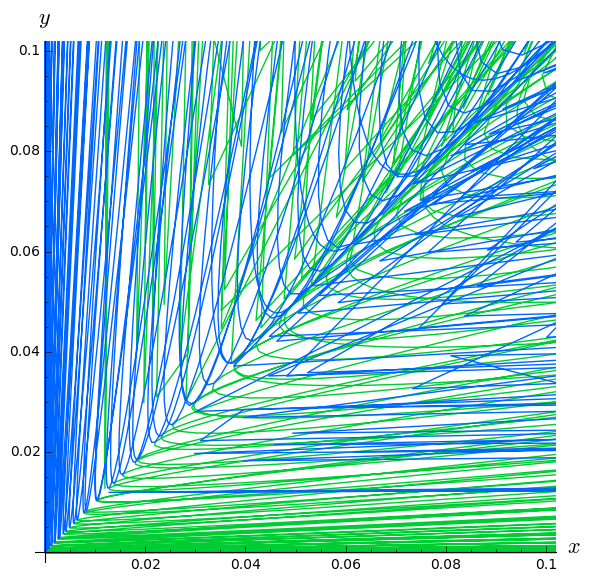
\includegraphics[width=1\textwidth]{plots/ch5_32_4curves2.png}
\vspace{-0.1cm}\caption{$\mathcal{N}_1(\sigma_\lambda)$ and $\mathcal{N}_1(\tau_\mu)$ in $[0, 0.1]^2$.}\label{curve}
\end{subfigure}
\hspace{2cm}
\begin{subfigure}{.28\linewidth}\centering
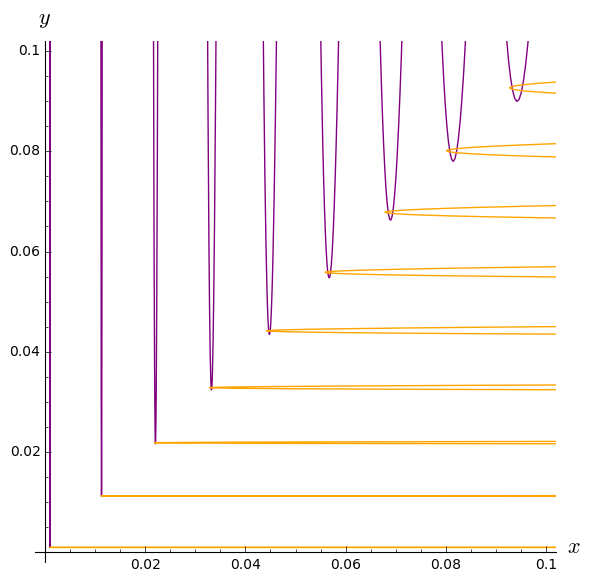
\includegraphics[width=1\textwidth]{plots/ch5_30_3curves5.png}
\vspace{-0.1cm}\caption{$f_2(\gamma_{\lambda})$ and $f_2(\delta_{\mu})$ in $[0, 0.1]^2$.}\label{curvef2}
\end{subfigure}
\end{figure}
\end{center}
\vspace{-1.5cm}
\end{alertblock}

%----------------------------------------------------------------------------------------
 
\vspace{-2cm}
 
\begin{columns}[t,totalwidth=\twocolwid] % Split up the two columns wide column again
 
\begin{column}{\onecolwid} % The first column within column 2 (column 2.1)
 
\vspace{-0.75cm}
%----------------------------------------------------------------------------------------
%       SECOND PROOF
%----------------------------------------------------------------------------------------
 
\begin{block}{About the second proof}
 
Let $f:=\HH\circ\GG\circ\FF:\R^2\to\R^2$, where:
\begin{equation*}\label{eq:secondMap}
\boxed{
\begin{aligned}
\FF(\x,\y) &= \big((\x\y-1)^2+\x^2,\ (\x\y-1)^2+\y^2\big),\\
\GG(\x,\y) &= \big(\x,\ \y(\x\y-2)^2+\x(\x\y-1)^2\big),\\
\HH(\x,\y) &= \big(\x(\x\y-2)^2+\tfrac{1}{2}\x\y^2,\ \y\big). \\
\end{aligned}
}
\end{equation*}
In this case the proof is conducted by inspecting at the images of the aforementioned polynomials.
 
\end{block}
 
%----------------------------------------------------------------------------------------
 
\end{column} % End of column 2.1
 
\begin{column}{\onecolwid} % The second column within column 2 (column 2.2)

\vspace{-0.75cm}
%----------------------------------------------------------------------------------------
%       COMPLEXITY ANALYSIS
%----------------------------------------------------------------------------------------
 
\begin{block}{Complexity analysis}

In this work we also present some new candidates whose images ``should be'' $\Qu$: $\mathcal{N}_1, \mathcal{N}_2$ and $\mathcal{N}_3$.
For the analysis, given a set of points we study how much time each map takes to compute the set of image points. We also examine which of the maps ``covers more area of $\Qu$'' given the same set of points.
 
\end{block}
 
%----------------------------------------------------------------------------------------
 
\end{column} % End of column 2.2
 
\end{columns} % End of the split of column 2
 
\end{column} % End of the second column
 
\begin{column}{\sepwid}\end{column} % Empty spacer column
 
\begin{column}{\onecolwid} % The third column
 

\begin{table}[t]
\begin{center}
\begin{tabular}{c |c| c | c | c}
&\negthinspace& Total degree & \begin{tabular}[c]{@{}c@{}}Total number\\of monomials\end{tabular} & \begin{tabular}[c]{@{}c@{}}Non-escalar\\complexity\end{tabular}\\ \hline 
\vspace{-1.4cm}&\negthinspace&&& \\ \hline
$g$ &\negthinspace& 56 & 167 & 13 \\ \hline
$f$ &\negthinspace& 72 &  350 & 11\\ \hline
{\scalebox{1.5}{$\FFF$}} &\negthinspace& 28 & 22 & 11\\ \hline
\vspace{-1.4cm}&\negthinspace&&& \\ \hline
$\mathcal{N}_1$&\negthinspace&16&24&10 \\ \hline
$\mathcal{N}_2$&\negthinspace&16&26&8 \\ \hline
$\mathcal{N}_3$&\negthinspace&20&26&13 \\	
\end{tabular}
\end{center}
\end{table}
\vspace{0.2cm}

In the analysis we start with some grids of points contained in a square, like a set of $4$ million points denoted as \scalebox{1.5}{$\PP$}$_6$.
We also use the families of curves that we mentioned before (and some others) in order to approach the positive half-axes.

%----------------------------------------------------------------------------------------
%       CONCLUSIONS
%----------------------------------------------------------------------------------------
 
\begin{block}{Conclusions}

Among the first 3 maps, the better one in terms of filling $\Qu$ seems to be $g$, but if we look at computation time \scalebox{1.5}{$\FFF$} is better.
Although Theorem 4 hasn't been proved for the new maps, they outstrip $g, f$ and \scalebox{1.5}{$\FFF$} on the tests. It is remarkable that for instance for $\mathcal{N}_1$, even when looking at $[0,0.1]^2$ the images of the curves stay really close to the positive half-axes (as we see on Figure \ref{curve}), whereas we don't see this behavior for $g$ and $f_2$ (Figures \ref{curveg} and \ref{curvef2}).
 
\end{block}

%----------------------------------------------------------------------------------------
%       REFERENCES
%----------------------------------------------------------------------------------------
 
\begin{block}{Some bibliography}
 
\footnotesize{
\begin{thebibliography}{ABR}

\bibitem[BCR]{bcr} J. Bochnak, M. Coste, M.-F. Roy: G\'eom\'etrie alg\'ebrique r\'eelle. \em Ergeb. Math. \em \textbf{12}, Springer-Verlag, Berlin, Heidelberg, New York (1987).
\vspace{0.2cm}

\bibitem[FG]{fg} J.F. Fernando, J.M. Gamboa: Polynomial images of $\R^n$. {\em J. Pure Appl. Algebra}, \textbf{179} (2003), 241--254.
\vspace{0.2cm}

\bibitem[FGU]{fgu} J.F. Fernando, J.M. Gamboa, C. Ueno: The open quadrant problem:
A topological proof.  A mathematical tribute to Professor Jos\'e Mar\'ia Montesinos. Departamento de Geometr\'ia y Topolog\'ia. Facultad de CC. Matem\'aticas UCM, (2016), 337--350.
\vspace{0.2cm}

\bibitem[FU1]{fu1} J.F. Fernando, C. Ueno: On the open quadrant as a polynomial image of $\R^2$ (revisited).
\vspace{0.2cm}

\bibitem[U]{u} C. Ueno: Im\'agenes polin\'omicas y regulares de espacios eucl\'\i deos. Ph.D. Thesis UCM, (2012).

\end{thebibliography}	}

\end{block}
 
%----------------------------------------------------------------------------------------
%       FURTHER READING
%----------------------------------------------------------------------------------------
 
\setbeamercolor{block alerted title}{fg=black,bg=ngreen} % Change the alert block title colors
\setbeamercolor{block alerted body}{fg=black,bg=white} % Change the alert block body colors
 
\begin{alertblock}{Further reading}
 
Full text and code can be found at \url{https://github.com/iipr/Final-Degree-Project}.
 
\end{alertblock}
 
 
%----------------------------------------------------------------------------------------
 
\end{column} % End of the third column
 
\end{columns} % End of all the columns in the poster
 
\end{frame} % End of the enclosing frame
 
\end{document}